\chapter{Wissensbasierte Systeme}

Wissensbasierte Systeme verwenden wissensbasierte Informationsverarbeitung, um L�sungen f�r Probleme zu berechnen. Diese Art der Informationsverarbeitung ist ein Paradigma, das eine strikte Trennung von Wissen und den zur L�sung des Problems erforderlichen Verarbeitungsmechanismen erfordert.

In einem klassischen System besteht ein Programm aus Programmen und Algorithmen. Ein wissensbasiertes System hingegen besteht aus symbolisch dargestelltem Wissen und Verarbeitungsmechanismen, um dieses Wissen zur Probleml�sung zu nutzen.

\begin{figure}[H]
    \centering
    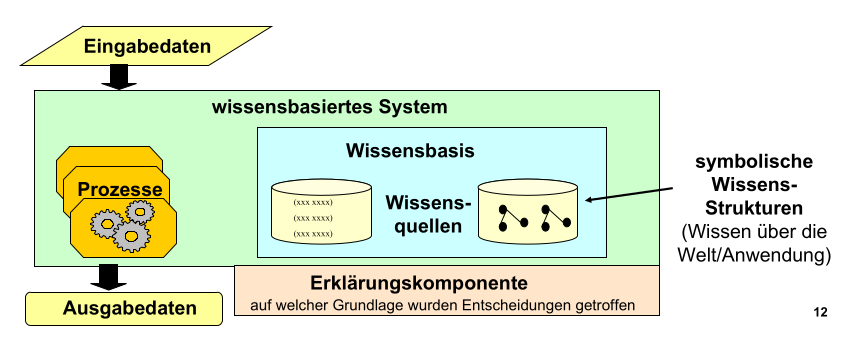
\includegraphics[width=\textwidth]{figures/kap6/anatomie-wbs.png}
    \caption{�berblick �ber ein wissensbasiertes System}
    \label{fig:overview-wbs}
\end{figure}

\section{Wissensdarstellung in wissensbasierten Systemen}

Wissensbasierte Informationsverarbeitung basiert auf der Vorstellung, dass viele Probleme nur l�sbar sind, wenn man Erfahrung mit dem Problem und den L�sungsm�glichkeiten daf�r hat. Dies wirft die Frage auf: Wie stellen wir Wissen so dar, dass es von Computern verstanden und zur Probleml�sung verwendet werden kann?

Wissen wird dabei als Klassen, Kategorien und Konzepte mit Hierarchien, Zusammensetzungen und Klassifikationen dargestellt. Dies ist eine ontologische Erfassung einer Anwendungsdom�ne bekannt. Diese Art der Datenmodellierung l�sst sich am besten mit einer Mindmap vergleichen (siehe Abb.~\ref{fig:mind-map-example}).

\begin{figure}[H]
    \centering
    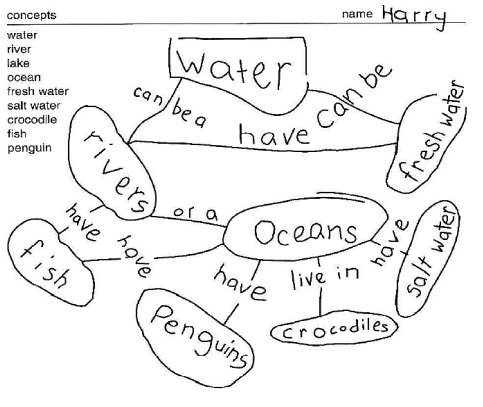
\includegraphics[width=0.52\textwidth]{figures/kap6/mind-map.png}
    \caption{Beispiel einer Mindmap von einem Grundsch�ler}
    \label{fig:mind-map-example}
\end{figure}

Diese Klassen, Kategorien und Konzepte werden letztlich in der Implementierung durch programmtypische Datenstrukturen wie Objekt-Arrays und Pointer abstrahiert (Abb.~\ref{fig:knowledge-darsetllung-ebenen}).

\begin{figure}[H]
    \centering
    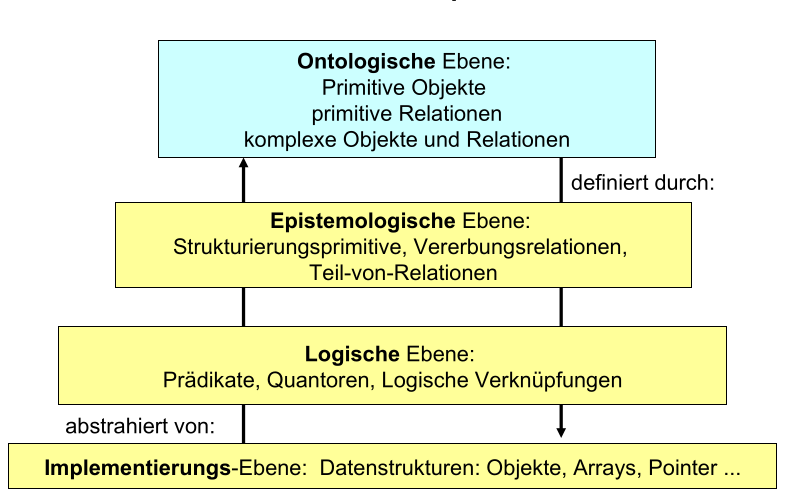
\includegraphics[width=0.8\textwidth]{figures/kap6/ebenen-wissendarstellung.png}
    \caption{Ebenen der Wissensrepr�sentation}
    \label{fig:knowledge-darsetllung-ebenen}
\end{figure}

Es gibt viele M�glichkeiten, Wissen explizit darzustellen. Eine Anwendung kann logikbasierte Ans�tze wie Fakten und Regeln verwenden. Andere k�nnen Rahmen und F�lle oder strukturierte Vererbungsnetze �hnlich objektorientierter Modelle verwenden.

\section{Schnittstelle zur Interaktion mit einem Wissenbassierten System}

Damit ein Benutzer mit einem wissensbasierten System interagieren kann, muss eine Schnittstelle vorhanden sein, die mindestens die folgenden Funktionen ausf�hren kann:

\begin{itemize}
    \item \textbf{Tell(WBS, knowledge-item):} F�ge dem System neues Wissen hinzu. z.B: "Die Welt ist Rund"
    \item \textbf{Ask(WBS, question):} Anfrage stellen. z.B: ist die Welt eine Kugel?
\end{itemize}

Allein durch die Verwendung dieser beiden Funktionen kann ein wissensbasiertes System verwendet werden, um Probleme innerhalb seiner Wissensbasis zu l�sen.

\section{Ans�tze zur Wissensverarbeitung}

Eine wichtige Komponente eines wissensbasierten Systems ist die Inferenzmaschine, die verwendet wird, um unsere Antworten auf Fragen zu finden. Es gibt viele Ans�tze f�r die Implementierung einer solchen Maschine zur Verarbeitung von vorhandenem Wissen.

\paragraph{Prinzip der Wissensabstraktion}

Diese Methode wird als induktive Inferenz bezeichnet: Ableitung allgemeiner Aussagen aus Spezialf�llen. z.B:

\begin{itemize}
    \item Beobachtung: Studenten Hans und Fritz haben ein Laptop
    \item Schlussfolgerung: Alle Studenten haben Laptops
\end{itemize}

\paragraph{Prinzip von Wissen �ber Wissensintegrit�t}

Diese Methode wird als deduktive Inferenz bezeichnet: Durch Erkennung von Regeln und Invarianzen aus formalen Beschreibungen wird explizites Wissen explizit gemacht. z.B:

\begin{itemize}
    \item Beobachtung: Aussage A ist wahr und Aussage B ist wahr.
    \item Schlussfolgerung: Auch die Aussage A oder B ist wahr.
\end{itemize}

\paragraph{Prinzip von Wissen �ber Kausalzusammenh�nge}

Diese Methode wird als abduktive Inferenz bezeichnet: Die Ursachen werden aus Beobachtungen abgeleitet: A ist der Grund daf�r, dass B passiert ist, wenn also B beobachtet wird, ist A passiert. z.B:

\begin{itemize}
    \item Beobachtung: Licht ist an.
    \item Schlussfolgerung: Lichtschalter ist auf Position ``Ein''.
\end{itemize}

\paragraph{Wissen �ber Analogien}

Diese Methode wird als analoge Inferenz bezeichnet: Neue Erkenntnisse werden aus bereits bekannten abgeleitet. z.B:

\begin{itemize}
    \item Beobachtung: durch ein dickes Rohr kann viel Wasser flie�en.
    \item Schlussfolgerung: durch ein dickes Kabel kann viel Strom flie�en.
\end{itemize}

\paragraph{Prinzip der Verwendung von empirischem Wissen}

Diese Methode wird als probabilistische Inferenz bezeichnet: Schlussfolgerung, dass eine Wirkung eintritt, basierend auf der Wahrscheinlichkeit, dass sie aufgrund der Situation eintritt. z.B:

\begin{itemize}
    \item Wenn 100 Personen im Raum sind, kann man davon ausgehen, dass mindestens zwei von ihnen denselben Geburtstag haben.
\end{itemize}

\paragraph{Prinzip der Verwendung von unscharfem Wissen}

Diese Methode wird als Fuzzy-Inferenz bezeichnet: Schlussfolgerungen auf der Grundlage der Wahrscheinlichkeit, dass ein Objekt zu einer Menge geh�rt. z.B:

\begin{itemize}
    \item Hans ist vierzig Jahre alt. Alte Menschen sind weise.
    \item Zugeh�rigkiet Hans zur Menge der jungen Menschen: 0.6
    \item Zugeh�rigkiet Hans zur Menge der alten Menschen: 0.4
    \item Ask: Ist Hans Weise? Antwort: Na ja, geht so
\end{itemize}

\section{Aufgaben beim Entwurf eines Wissenbassierten Systems}

Es ist es wichtig, von Anfang an herauszufinden, welche Arten von Wissen es zu erwerben gilt und wie diese repr�sentiert und gespeichert werden. Daneben muss auch entschieden werden, welche Inferenzmechanismen verwendet werden sollen.

Dann stellt sich die Frage, wie die Wissensbasis gef�llt werden soll. Dazu gibt es einfache Methoden, z. B. indem man einen Experten dazu bringt, sein Wissen mit einem Texteditor, einem Formular oder einem Mikrofon einzugeben. Es gibt aber auch komplexere Ans�tze wie die Entwicklung einer Schnittstelle zur Umwandlung von Datenbankinhalten in ein Format, das von einem wissensbasierten System verarbeitet werden kann, oder die Extraktion neuen Wissens mit Hilfe k�nstlicher neuronaler Netze. 

\section{Vertiefung: The Bitter Lesson}

In dem kurzen Essay von Richard Sutton, einem kanadischen Informatiker, diskutiert er den seiner Meinung nach gr��ten Fehler der KI-Forschung der letzten 70 Jahre. Er argumentiert, dass die KI-Forschung durch einen zu starken Fokus auf die Verwendung von Ans�tzen des ``menschlichen Wissens'' anstelle der Verwendung von Rechenleistung behindert wurde.

Als Beispiel verwies er auf das Jahr 1997, als Kasparov, Schachweltmeister, von einem Computer besiegt wurde, der Deep Search mit spezieller Hard- und Software verwendete, anstatt das menschliche Verst�ndnis der besonderen Natur des Schachs zu nutzen. Diese Methode wurde von der Mehrheit der Computerschachforscher abgelehnt, die entt�uscht waren, dass das System keine Methoden verwendete, die auf menschlichem Input basierten, um zu gewinnen.

�hnliche Situationen gab es bei der Entwicklung von Computer Go, Spracherkennung und Computer Vision. Dabei kamen zun�chst solche Ans�tze: die Besonderheiten des Spiels bei Go, die Kenntnis von W�rtern und Ph�nomenen f�r die Spracherkennung oder die Suche nach Kanten und Zylindern im Computer Vision. Am Ende wurde all dies jedoch zugunsten neuerer Methoden verworfen, die sich die rohe Rechenleistung zunutze machen, die aufgrund des Mooresschen Gesetzes zur Verf�gung gestellt wurde.

Die bitteren Lehren laut Richard Sutton sind, dass die Leistungsf�higkeit von Allzweckmethoden, die mit zunehmender Rechenleistung weiter skalieren, nicht untersch�tzt werden sollte und dass sich die KI-Forschung darauf konzentrieren sollte, KI-Agenten zu erm�glichen, herauszufinden, wie sie die Au�enwelt verstehen k�nnen. und der KI keine bestimmte Denkweise aufzuzwingen.